\chapter{Recurrent Neural Networks} \label{sec:chapterRNN}

\minitoc

\section{Introduction}

\yinipar{\fontsize{60pt}{72pt}\usefont{U}{Kramer}{xl}{n}I}n this chapter, we review a third kind of Neural Network architecture: Recurrent Neural Networks\cite{GravesA2016}. By contrast with the CNN, this kind of network introduces a real architecture novelty : instead of forwarding only in a "spatial" direction, the data are also forwarded in a new -- time dependent -- direction. We will present the first Recurrent Neural Network (RNN) architecture, as well as the current most popular one: the Long Short Term Memory (LSTM) Neural Network.

\section{RNN-LSTM architecture}

\subsection{Forward pass in a RNN-LSTM}

In figure \ref{fig:1}, we present the RNN architecture in a schematic way

\begin{figure}[H]
\begin{center}
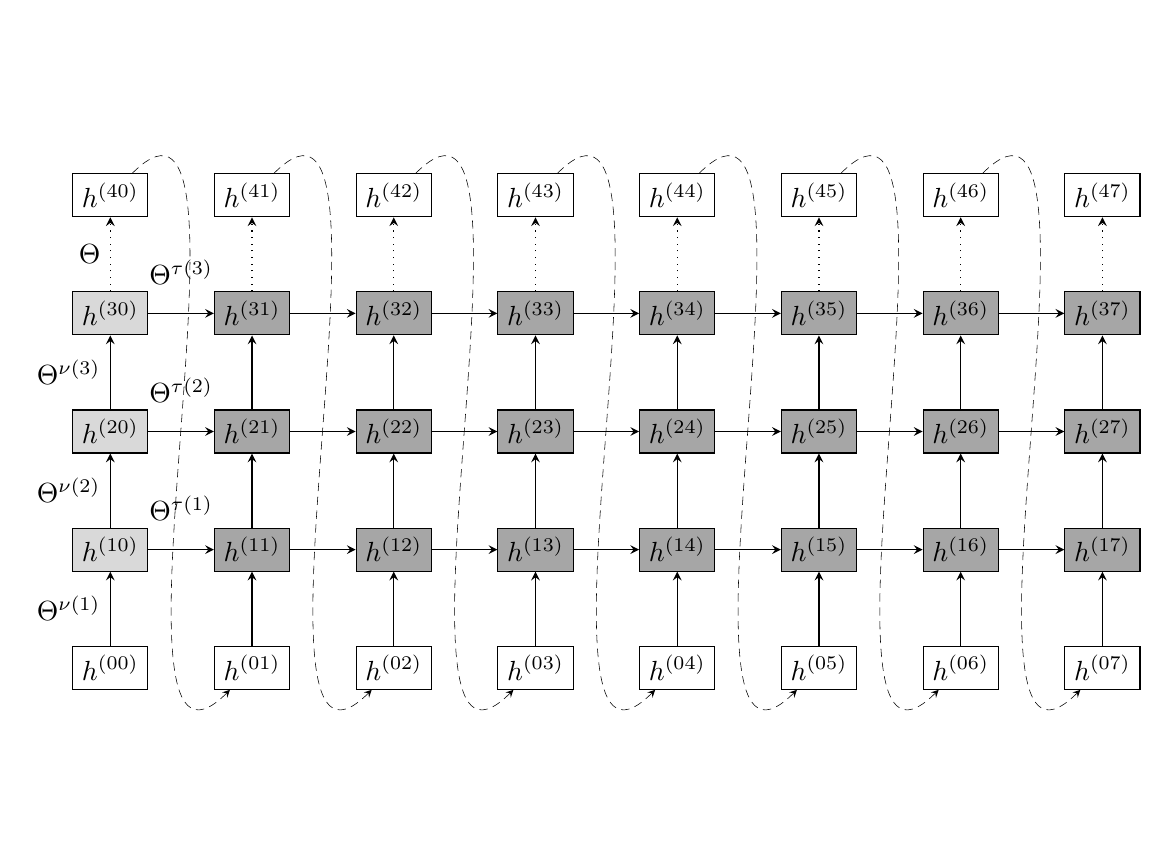
\begin{tikzpicture}
\node at (0,0) [rectangle,draw,fill=gray!0!white] (h00) {$h^{(00)}$};
\node at (0,1.5) [rectangle,draw,fill=gray!30!white] (h01) {$h^{(10)}$};
\node at (0,3) [rectangle,draw,fill=gray!30!white] (h02) {$h^{(20)}$};
\node at (0,4.5) [rectangle,draw,fill=gray!30!white] (h03) {$h^{(30)}$};
\node at (0,6) [rectangle,draw,fill=gray!0!white] (h04) {$h^{(40)}$};
%
\node at (1.8,0) [rectangle,draw,fill=gray!0!white] (h10) {$h^{(01)}$};
\node at (1.8,1.5) [rectangle,draw,fill=gray!70!white] (h11) {$h^{(11)}$};
\node at (1.8,3) [rectangle,draw,fill=gray!70!white] (h12) {$h^{(21)}$};
\node at (1.8,4.5) [rectangle,draw,fill=gray!70!white] (h13) {$h^{(31)}$};
\node at (1.8,6) [rectangle,draw,fill=gray!0!white] (h14) {$h^{(41)}$};
%
\node at (3.6,0) [rectangle,draw,fill=gray!0!white] (h20) {$h^{(02)}$};
\node at (3.6,1.5) [rectangle,draw,fill=gray!70!white] (h21) {$h^{(12)}$};
\node at (3.6,3) [rectangle,draw,fill=gray!70!white] (h22) {$h^{(22)}$};
\node at (3.6,4.5) [rectangle,draw,fill=gray!70!white] (h23) {$h^{(32)}$};
\node at (3.6,6) [rectangle,draw,fill=gray!0!white] (h24) {$h^{(42)}$};
%
\node at (5.4,0) [rectangle,draw,fill=gray!0!white] (h30) {$h^{(03)}$};
\node at (5.4,1.5) [rectangle,draw,fill=gray!70!white] (h31) {$h^{(13)}$};
\node at (5.4,3) [rectangle,draw,fill=gray!70!white] (h32) {$h^{(23)}$};
\node at (5.4,4.5) [rectangle,draw,fill=gray!70!white] (h33) {$h^{(33)}$};
\node at (5.4,6) [rectangle,draw,fill=gray!0!white] (h34) {$h^{(43)}$};
%
\node at (7.2,0) [rectangle,draw,fill=gray!0!white] (h40) {$h^{(04)}$};
\node at (7.2,1.5) [rectangle,draw,fill=gray!70!white] (h41) {$h^{(14)}$};
\node at (7.2,3) [rectangle,draw,fill=gray!70!white] (h42) {$h^{(24)}$};
\node at (7.2,4.5) [rectangle,draw,fill=gray!70!white] (h43) {$h^{(34)}$};
\node at (7.2,6) [rectangle,draw,fill=gray!0!white] (h44) {$h^{(44)}$};
%
\node at (9,0) [rectangle,draw,fill=gray!0!white] (h50) {$h^{(05)}$};
\node at (9,1.5) [rectangle,draw,fill=gray!70!white] (h51) {$h^{(15)}$};
\node at (9,3) [rectangle,draw,fill=gray!70!white] (h52) {$h^{(25)}$};
\node at (9,4.5) [rectangle,draw,fill=gray!70!white] (h53) {$h^{(35)}$};
\node at (9,6) [rectangle,draw,fill=gray!0!white] (h54) {$h^{(45)}$};
%
\node at (10.8,0) [rectangle,draw,fill=gray!0!white] (h60) {$h^{(06)}$};
\node at (10.8,1.5) [rectangle,draw,fill=gray!70!white] (h61) {$h^{(16)}$};
\node at (10.8,3) [rectangle,draw,fill=gray!70!white] (h62) {$h^{(26)}$};
\node at (10.8,4.5) [rectangle,draw,fill=gray!70!white] (h63) {$h^{(36)}$};
\node at (10.8,6) [rectangle,draw,fill=gray!0!white] (h64) {$h^{(46)}$};
%
\node at (12.6,0) [rectangle,draw,fill=gray!0!white] (h70) {$h^{(07)}$};
\node at (12.6,1.5) [rectangle,draw,fill=gray!70!white] (h71) {$h^{(17)}$};
\node at (12.6,3) [rectangle,draw,fill=gray!70!white] (h72) {$h^{(27)}$};
\node at (12.6,4.5) [rectangle,draw,fill=gray!70!white] (h73) {$h^{(37)}$};
\node at (12.6,6) [rectangle,draw,fill=gray!0!white] (h74) {$h^{(47)}$};
%
%
\draw[-stealth] (h00) -- node[pos=0.5,anchor=east,scale=1] {$\Theta^{\nu(1)}$} (h01);
\draw[-stealth] (h01) -- node[pos=0.5,anchor=east,scale=1] {$\Theta^{\nu(2)}$} (h02);
\draw[-stealth] (h02) -- node[pos=0.5,anchor=east,scale=1] {$\Theta^{\nu(3)}$} (h03);
\draw[dotted,-stealth] (h03) -- node [pos=0.5,anchor = east] {$\Theta$} (h04);
%
\draw[-stealth] (h10) -- (h11);
\draw[-stealth] (h11) -- (h12);
\draw[-stealth] (h12) -- (h13);
\draw[dotted,-stealth] (h13) -- (h14);
%
\draw[-stealth] (h20) -- (h21);
\draw[-stealth] (h21) -- (h22);
\draw[-stealth] (h22) -- (h23);
\draw[dotted,-stealth] (h23) -- (h24);
%
\draw[-stealth] (h30) -- (h31);
\draw[-stealth] (h31) -- (h32);
\draw[-stealth] (h32) -- (h33);
\draw[dotted,-stealth] (h33) -- (h34);
%
\draw[-stealth] (h40) -- (h41);
\draw[-stealth] (h41) -- (h42);
\draw[-stealth] (h42) -- (h43);
\draw[dotted,-stealth] (h43) -- (h44);
%
\draw[-stealth] (h50) -- (h51);
\draw[-stealth] (h51) -- (h52);
\draw[-stealth] (h52) -- (h53);
\draw[dotted,-stealth] (h53) -- (h54);
%
\draw[-stealth] (h60) -- (h61);
\draw[-stealth] (h61) -- (h62);
\draw[-stealth] (h62) -- (h63);
\draw[dotted,-stealth] (h63) -- (h64);
%
\draw[-stealth] (h70) -- (h71);
\draw[-stealth] (h71) -- (h72);
\draw[-stealth] (h72) -- (h73);
\draw[dotted,-stealth] (h73) -- (h74);
%
\draw[-stealth] (h01) --   node[pos=0.5,above=7pt,scale=1] {$\Theta^{\tau(1)}$} (h11);
\draw[-stealth] (h11) -- (h21);
\draw[-stealth] (h21) -- (h31);
\draw[-stealth] (h31) -- (h41);
\draw[-stealth] (h41) -- (h51);
\draw[-stealth] (h51) -- (h61);
\draw[-stealth] (h61) -- (h71);
%
\draw[-stealth] (h02) -- node[pos=0.5,above=7pt,scale=1] {$\Theta^{\tau(2)}$} (h12);
\draw[-stealth] (h12) -- (h22);
\draw[-stealth] (h22) -- (h32);
\draw[-stealth] (h32) -- (h42);
\draw[-stealth] (h42) -- (h52);
\draw[-stealth] (h52) -- (h62);
\draw[-stealth] (h62) -- (h72);
%
\draw[-stealth] (h03) -- node[pos=0.5,above=7pt,scale=1] {$\Theta^{\tau(3)}$} (h13);
\draw[-stealth] (h13) -- (h23);
\draw[-stealth] (h23) -- (h33);
\draw[-stealth] (h33) -- (h43);
\draw[-stealth] (h43) -- (h53);
\draw[-stealth] (h53) -- (h63);
\draw[-stealth] (h63) -- (h73);
%
\draw[very thin,densely dashed,-stealth] (h04) to[out=45,in=225] (h10);
\draw[very thin,densely dashed,-stealth] (h14) to[out=45,in=225] (h20);
\draw[very thin,densely dashed,-stealth] (h24) to[out=45,in=225] (h30);
\draw[very thin,densely dashed,-stealth] (h34) to[out=45,in=225] (h40);
\draw[very thin,densely dashed,-stealth] (h44) to[out=45,in=225] (h50);
\draw[very thin,densely dashed,-stealth] (h54) to[out=45,in=225] (h60);
\draw[very thin,densely dashed,-stealth] (h64) to[out=45,in=225] (h70);
\end{tikzpicture}
\caption{\label{fig:RNN architecture}RNN architecture, with data propagating both in "space" and in "time". In our example, the time dimension is of size 8 while the "spatial" one is of size 4.}
\end{center}
\end{figure}

The real novelty of this type of neural network is that the fact that we are trying to predict a time series is encoded in the very architecture of the network. RNN have first been introduced mostly to predict the next words in a sentence (classification task), hence the notion of ordering in time of the prediction. But this kind of network architecture can also be applied to regression problems. Among others things one can think of stock prices evolution, or temperature forecasting. In contrast to the precedent neural networks that we introduced, where we defined (denoting $\nu$ as in previous chapters the layer index in the spatial direction)
\begin{align}
a^{(t)(\nu)}_{f}&= \text{ Weight Averaging } \left(h^{(t)(\nu)}_{f}\right)\;,\notag\\
%
h^{(t)(\nu+1)}_{f}&= \text{ Activation function } \left(a^{(t)(\nu)}_{f}\right)\;,
\end{align}
we now have the hidden layers that are indexed by both a "spatial" and a "temporal" index (with $T$ being the network dimension in this new direction), and the general philosophy of the RNN is (now the $a$ is usually characterized by a $c$ for cell state, this denotation, trivial for the basic RNN architecture will make more sense when we talk about LSTM networks)
\begin{align}
c^{(t)(\nu \tau )}_{f}&= \text{ Weight Averaging } \left(h^{(t)(\nu \tau-1)}_{f},h^{(t)(\nu-1\tau)}_{f}\right)\;,\notag\\
%
h^{(t)(\nu\tau)}_{f}&= \text{ Activation function } \left(c^{(t)(\nu \tau)}_{f}\right)\;,
\end{align}

\subsection{Backward pass in a RNN-LSTM}

The backward pass in a RNN-LSTM has to respect a certain time order, as illustrated in the following figure.

\begin{figure}[H]
\begin{center}
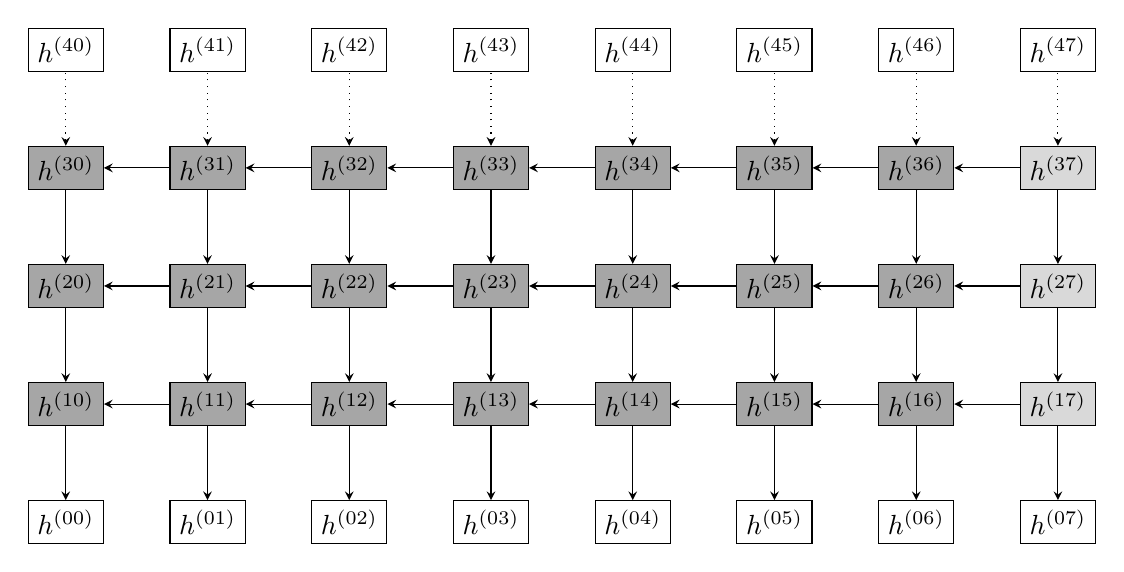
\begin{tikzpicture}
\node at (0,0) [rectangle,draw,fill=gray!0!white] (h00) {$h^{(00)}$};
\node at (0,1.5) [rectangle,draw,fill=gray!70!white] (h01) {$h^{(10)}$};
\node at (0,3) [rectangle,draw,fill=gray!70!white] (h02) {$h^{(20)}$};
\node at (0,4.5) [rectangle,draw,fill=gray!70!white] (h03) {$h^{(30)}$};
\node at (0,6) [rectangle,draw,fill=gray!0!white] (h04) {$h^{(40)}$};
%
\node at (1.8,0) [rectangle,draw,fill=gray!0!white] (h10) {$h^{(01)}$};
\node at (1.8,1.5) [rectangle,draw,fill=gray!70!white] (h11) {$h^{(11)}$};
\node at (1.8,3) [rectangle,draw,fill=gray!70!white] (h12) {$h^{(21)}$};
\node at (1.8,4.5) [rectangle,draw,fill=gray!70!white] (h13) {$h^{(31)}$};
\node at (1.8,6) [rectangle,draw,fill=gray!0!white] (h14) {$h^{(41)}$};
%
\node at (3.6,0) [rectangle,draw,fill=gray!0!white] (h20) {$h^{(02)}$};
\node at (3.6,1.5) [rectangle,draw,fill=gray!70!white] (h21) {$h^{(12)}$};
\node at (3.6,3) [rectangle,draw,fill=gray!70!white] (h22) {$h^{(22)}$};
\node at (3.6,4.5) [rectangle,draw,fill=gray!70!white] (h23) {$h^{(32)}$};
\node at (3.6,6) [rectangle,draw,fill=gray!0!white] (h24) {$h^{(42)}$};
%
\node at (5.4,0) [rectangle,draw,fill=gray!0!white] (h30) {$h^{(03)}$};
\node at (5.4,1.5) [rectangle,draw,fill=gray!70!white] (h31) {$h^{(13)}$};
\node at (5.4,3) [rectangle,draw,fill=gray!70!white] (h32) {$h^{(23)}$};
\node at (5.4,4.5) [rectangle,draw,fill=gray!70!white] (h33) {$h^{(33)}$};
\node at (5.4,6) [rectangle,draw,fill=gray!0!white] (h34) {$h^{(43)}$};
%
\node at (7.2,0) [rectangle,draw,fill=gray!0!white] (h40) {$h^{(04)}$};
\node at (7.2,1.5) [rectangle,draw,fill=gray!70!white] (h41) {$h^{(14)}$};
\node at (7.2,3) [rectangle,draw,fill=gray!70!white] (h42) {$h^{(24)}$};
\node at (7.2,4.5) [rectangle,draw,fill=gray!70!white] (h43) {$h^{(34)}$};
\node at (7.2,6) [rectangle,draw,fill=gray!0!white] (h44) {$h^{(44)}$};
%
\node at (9,0) [rectangle,draw,fill=gray!0!white] (h50) {$h^{(05)}$};
\node at (9,1.5) [rectangle,draw,fill=gray!70!white] (h51) {$h^{(15)}$};
\node at (9,3) [rectangle,draw,fill=gray!70!white] (h52) {$h^{(25)}$};
\node at (9,4.5) [rectangle,draw,fill=gray!70!white] (h53) {$h^{(35)}$};
\node at (9,6) [rectangle,draw,fill=gray!0!white] (h54) {$h^{(45)}$};
%
\node at (10.8,0) [rectangle,draw,fill=gray!0!white] (h60) {$h^{(06)}$};
\node at (10.8,1.5) [rectangle,draw,fill=gray!70!white] (h61) {$h^{(16)}$};
\node at (10.8,3) [rectangle,draw,fill=gray!70!white] (h62) {$h^{(26)}$};
\node at (10.8,4.5) [rectangle,draw,fill=gray!70!white] (h63) {$h^{(36)}$};
\node at (10.8,6) [rectangle,draw,fill=gray!0!white] (h64) {$h^{(46)}$};
%
\node at (12.6,0) [rectangle,draw,fill=gray!0!white] (h70) {$h^{(07)}$};
\node at (12.6,1.5) [rectangle,draw,fill=gray!30!white] (h71) {$h^{(17)}$};
\node at (12.6,3) [rectangle,draw,fill=gray!30!white] (h72) {$h^{(27)}$};
\node at (12.6,4.5) [rectangle,draw,fill=gray!30!white] (h73) {$h^{(37)}$};
\node at (12.6,6) [rectangle,draw,fill=gray!0!white] (h74) {$h^{(47)}$};
%
%
\draw[stealth-] (h00) -- (h01);
\draw[stealth-] (h01) -- (h02);
\draw[stealth-] (h02) -- (h03);
\draw[dotted,stealth-] (h03) -- (h04);
%
\draw[stealth-] (h10) -- (h11);
\draw[stealth-] (h11) -- (h12);
\draw[stealth-] (h12) -- (h13);
\draw[dotted,stealth-] (h13) -- (h14);
%
\draw[stealth-] (h20) -- (h21);
\draw[stealth-] (h21) -- (h22);
\draw[stealth-] (h22) -- (h23);
\draw[dotted,stealth-] (h23) -- (h24);
%
\draw[stealth-] (h30) -- (h31);
\draw[stealth-] (h31) -- (h32);
\draw[stealth-] (h32) -- (h33);
\draw[dotted,stealth-] (h33) -- (h34);
%
\draw[stealth-] (h40) -- (h41);
\draw[stealth-] (h41) -- (h42);
\draw[stealth-] (h42) -- (h43);
\draw[dotted,stealth-] (h43) -- (h44);
%
\draw[stealth-] (h50) -- (h51);
\draw[stealth-] (h51) -- (h52);
\draw[stealth-] (h52) -- (h53);
\draw[dotted,stealth-] (h53) -- (h54);
%
\draw[stealth-] (h60) -- (h61);
\draw[stealth-] (h61) -- (h62);
\draw[stealth-] (h62) -- (h63);
\draw[dotted,stealth-] (h63) -- (h64);
%
\draw[stealth-] (h70) -- (h71);
\draw[stealth-] (h71) -- (h72);
\draw[stealth-] (h72) -- (h73);
\draw[dotted,stealth-] (h73) -- (h74);
%
\draw[stealth-] (h01) -- (h11);
\draw[stealth-] (h11) -- (h21);
\draw[stealth-] (h21) -- (h31);
\draw[stealth-] (h31) -- (h41);
\draw[stealth-] (h41) -- (h51);
\draw[stealth-] (h51) -- (h61);
\draw[stealth-] (h61) -- (h71);
%
\draw[stealth-] (h02) -- (h12);
\draw[stealth-] (h12) -- (h22);
\draw[stealth-] (h22) -- (h32);
\draw[stealth-] (h32) -- (h42);
\draw[stealth-] (h42) -- (h52);
\draw[stealth-] (h52) -- (h62);
\draw[stealth-] (h62) -- (h72);
%
\draw[stealth-] (h03) -- (h13);
\draw[stealth-] (h13) -- (h23);
\draw[stealth-] (h23) -- (h33);
\draw[stealth-] (h33) -- (h43);
\draw[stealth-] (h43) -- (h53);
\draw[stealth-] (h53) -- (h63);
\draw[stealth-] (h63) -- (h73);
\end{tikzpicture}
\caption{\label{fig:rnnback}Architecture taken, backward pass. Here what cannot compute the gradient of a layer without having computed the ones that flow into it}
\end{center}
\end{figure}


With this in mind, let us now see in details the implementation of a RNN and its advanced cousin, the Long Short Term Memory (LSTM)-RNN.

\section{Extreme Layers and loss function}

These part of the RNN-LSTM networks just experiences trivial modifications. Let us see them

\subsection{Input layer}

In a RNN-LSTM, the input layer is recursively defined as 
\begin{align}
h^{(t)(0\tau+1)}_{f}&=\left(\tilde{h}^{(t)(0\tau)}_{f},h^{(t)(N-1\tau)}_{f}\right)\;.
\end{align}
where $\tilde{h}^{(t)(0\tau)}_{f}$ is $h^{(t)(0\tau)}_{f}$ with the first time column removed.

\subsection{Output layer }

The output layer of a RNN-LSTM reads
\begin{align}
h^{(t)(N\tau)}_{f}&=o\left(\sum_{f'=0}^{F_{N-1}-1}\Theta^f_{f'} h^{(t)(N-1\tau)}_{f}\right)\;,
\end{align}
where the output function $o$ is as for FNN's and CNN's is either the identity (regression task) or the cross-entropy function (classification task).

\subsection{Loss function}

The loss function for a regression task reads
\begin{align}
J(\Theta)&=\frac{1}{2T_{{\rm mb}}}\sum_{t=0}^{T_{{\rm mb}}-1}\sum_{\tau=0}^{T-1}\sum_{f=0}^{F_N-1}
%
\left(h^{(t)( N\tau)}_f-y^{(t)(\tau)}_f\right)^2\;.
\end{align}
and for a classification task
\begin{align}
J(\Theta)&=-\frac{1}{T_{{\rm mb}}}\sum_{t=0}^{T_{{\rm mb}}-1}\sum_{\tau=0}^{T-1}\sum_{c=0}^{C-1}
%
\delta^{c}_{y^{(t)(\tau)}_c}  \ln \left(h^{(t)( N\tau)}_f\right)\;.
\end{align}


\section{RNN specificities}

\subsection{RNN structure} \label{sec:rnnstructure}

RNN is the most basic architecture that takes -- thanks to the way it is built in -- into account the time structure of the data to be predicted. Zooming on one hidden layer of \ref{fig:RNN architecture}, here is what we see for a simple Recurrent Neural Network.

\begin{figure}[H]
\begin{center}
\begin{tikzpicture}
\node[] at (0,0) {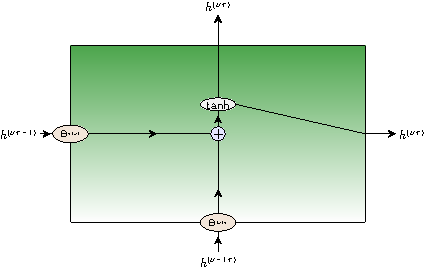
\includegraphics[scale=1.5]{RNN_structure}};
\end{tikzpicture}
\caption{\label{fig:RNN hidden unit}RNN hidden unit details}
\end{center}
\end{figure}

And here is how the output of the hidden layer represented in \ref{fig:RNN hidden unit} enters into the subsequent hidden units

\begin{figure}[H]
\begin{center}
\begin{tikzpicture}
\node[] at (0,0) {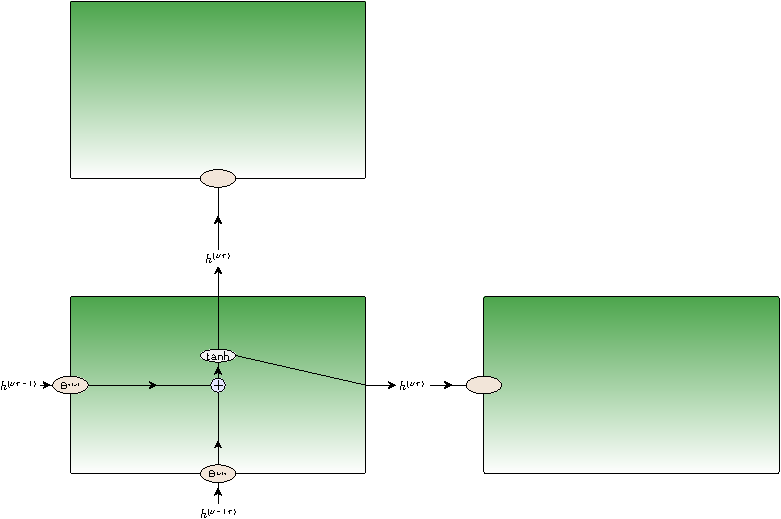
\includegraphics[scale=0.8]{RNN_structure-tot}};
\end{tikzpicture}
\caption{\label{fig:RNN interaction}How the RNN hidden unit interact with each others}
\end{center}
\end{figure}


Lest us now mathematically express what is represented in figures \ref{fig:RNN hidden unit} and \ref{fig:RNN interaction}.

\subsection{Forward pass in a RNN}

 In a RNN, the update rules read for the first time slice (spatial layer at the extreme left of figure \ref{fig:RNN architecture})
 
\begin{align}
h^{(t)(\nu\tau)}_f&=\tanh\left(\sum_{f'=0}^{F_{{\nu-1}}-1}\Theta^{\nu(\nu)f}_{f'}
%
h^{(t)(\nu-1\tau)}_{f'}\right)\;,
\end{align}

and for the other ones

\begin{align}
h^{(t)(\nu\tau)}_f&=\tanh\left(\sum_{f'=0}^{F_{{\nu-1}}-1}\Theta^{\nu(\nu)f}_{f'}
%
h^{(t)(\nu-1\tau)}_{f'}+\sum_{f'=0}^{F_{{\nu}}-1}\Theta^{\tau(\nu)f}_{f'}
%
h^{(t)(\nu\tau-1)}_{f'}\right)\;.
\end{align}

\subsection{Backpropagation in a RNN}

The backpropagation philosophy will remain unchanged : find the error rate updates, from which one can deduce the weight updates. But as for the hidden layers, the $\delta$ now have both a spatial and a temporal component. We will thus have to compute 
\begin{align}
\delta^{(t)( \nu\tau)}_f&=\frac{\delta}{\delta h^{(t)( \nu+1\tau)}_f }J(\Theta)\;,
\end{align}
to deduce
\begin{align}
\Delta^{\Theta{\rm index}f}_{f'}&=\frac{\delta}{\delta \Delta^{\Theta{\rm index}f}_{f'} }J(\Theta)\;,
\end{align}
where the index can either be nothing (weights of the output layers), $\nu(\nu)$ (weights between two spatially connected layers) or  $\tau(\nu)$ (weights between two temporally connected layers). First, it is easy to compute (in the same way as in chapter 1 for FNN) for the MSE loss function
\begin{align}
\delta^{(t)(N-1\tau)}_f&= \frac{1}{T_{{\rm mb}}}\left(h_{f}^{(t)(N\tau)}-y_f^{(t)(\tau)}\right)\;,
\end{align}
and for the cross entropy loss function
\begin{align}
\delta^{(t)(N-1)}_{f}&= \frac{1}{T_{{\rm mb}}}\left(h_{f}^{(t)(N\tau)}-\delta^f_{y^{(t)(\tau)}}\right)\;.
\end{align}
Calling 
\begin{align}
\mathcal{T}_{f}^{(t)(\nu\tau)}&=1-\left(h_{f}^{(t)(\nu\tau)}\right)^2\;,
\end{align}
and
\begin{align}
\mathcal{H}^{(t')(\nu\tau)_a}_{ff'}&=\mathcal{T}^{(t')(\nu+1\tau)}_{f'}\Theta^{a(\nu+1)f'}_{f}\;,
\end{align}
we show in appendix \ref{sec:rnnappenderrorrate} that (if $\tau+1$ exists, otherwise the second term is absent)
\begin{align}
\delta^{(t)(\nu-1\tau)}_f&= 
%
\sum_{t'=0}^{T_{{\rm mb}}}J^{(tt')(\nu\tau)}_f\sum_{\epsilon=0}^{1}\sum_{f'=0}^{F_{\nu+1-\epsilon}-1}
%
\mathcal{H}^{(t')(\nu-\epsilon\tau+\epsilon)_{b_\epsilon}}_{ff'}\delta^{(t')(\nu-\epsilon\tau+\epsilon)}_{f'}\;.
\end{align}
where $b_0=\nu$ and $b_1=\tau$.

\subsection{Weight and coefficient updates in a RNN}

To complete the backpropagation algorithm, we need

\begin{align}
&\Delta^{\nu(\nu)f}_{f'}\;,&
%
&\Delta^{\tau(\nu)f}_{f'}\;,&
%
&\Delta^{f}_{f'}\;,&
%
&\Delta^{\beta(\nu \tau)}_{f}\;,&
%
&\Delta^{\gamma(\nu \tau)}_{f}\;.
\end{align}

We show in appendix \ref{sec:rnncoefficient} that

\begin{align}
\Delta^{\nu(\nu-)f}_{f'}&=\sum_{\tau=0}^{T-1}\sum_{t=0}^{T_{{\rm mb}}-1}
%
\mathcal{T}^{(t)(\nu\tau)}_{f}\delta^{(t)(\nu-1\tau)}_{f}h^{(t)(\nu-1\tau)}_{f'}\;,\\
%
\Delta^{\tau(\nu)f}_{f'}&=\sum_{\tau=1}^{T-1}\sum_{t=0}^{T_{{\rm mb}}-1}
%
\mathcal{T}^{(t)(\nu\tau)}_{f}\delta^{(t)(\nu-1\tau)}_{f}h^{(t)(\nu\tau-1)}_{f'}\;,\\
%
\Delta^{f}_{f'}&=\sum_{\tau=0}^{T-1}\sum_{t=0}^{T_{{\rm mb}}-1} h^{(t)(N-1\tau)}_{f'}\delta^{(t)(N-1\tau)}_{f}\;,\\
%
\Delta^{\beta(\nu \tau)}_{f}&=\sum_{t=0}^{T_{{\rm mb}}-1}\sum_{\epsilon=0}^{1}\sum_{f'=0}^{F_{\nu+1-\epsilon}-1}
%
\mathcal{H}^{(t')(\nu-\epsilon\tau+\epsilon)_{b_\epsilon}}_{ff'}\delta^{(t')(\nu-\epsilon\tau+\epsilon)}_{f'}\;,\\
%
\Delta^{\gamma(\nu \tau)}_{f}&=\sum_{t=0}^{T_{{\rm mb}}-1}\tilde{h}^{(t)(\nu\tau)}_{f}\sum_{\epsilon=0}^{1}\sum_{f'=0}^{F_{\nu+1-\epsilon}-1}
%
\mathcal{H}^{(t')(\nu-\epsilon\tau+\epsilon)_{b_\epsilon}}_{ff'}\delta^{(t')(\nu-\epsilon\tau+\epsilon)}_{f'}\;.
\end{align}

\section{LSTM specificities}


\subsection{LSTM structure}


In a Long Short Term Memory Neural Network\cite{Gers:2000:LFC:1121912.1121915}, the state of a given unit is not directly determined by its left and bottom neighbours. Instead, a cell state is updated for each hidden unit, and the output of this unit is a probe of the cell state. This formulation might seem puzzling at first, but it is philosophically similar to the ResNet approach that we briefly encounter in the appendix of chapter \ref{sec:chapterFNN}: instead of trying to fit an input with a complicated function, we try to fit tiny variation of the input, hence allowing the gradient to flow in a smoother manner in the network. In the LSTM network, several gates are thus introduced : the input gate $i^{(t)(\nu\tau)}_f$ determines if we allow new information $g^{(t)(\nu\tau)}_f$ to enter into the cell state. The  output gate $o^{(t)(\nu\tau)}_f$ determines if we set or not the output hidden value to $0$, or really probes the current cell state. Finally, the forget state $f^{(t)(\nu\tau)}_f$ determines if we forget or not the past cell state. All theses concepts are illustrated on the figure \ref{fig:Lstm1}, which is the LSTM counterpart of the RNN structure of section \ref{sec:rnnstructure}. This diagram will be explained in details in the next section.

\begin{figure}[H]
\begin{center}
\begin{tikzpicture}
\node[] at (0,0) {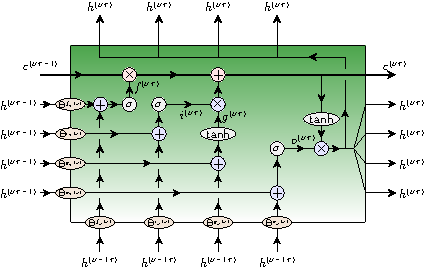
\includegraphics[scale=1.7]{LSTM_structure}};
\end{tikzpicture}
\caption{\label{fig:Lstm1}LSTM hidden unit details}
\end{center}
\end{figure}

In a LSTM, the different hidden units interact in the following way

\begin{figure}[H]
\begin{center}
\begin{tikzpicture}
\node[] at (0,0) {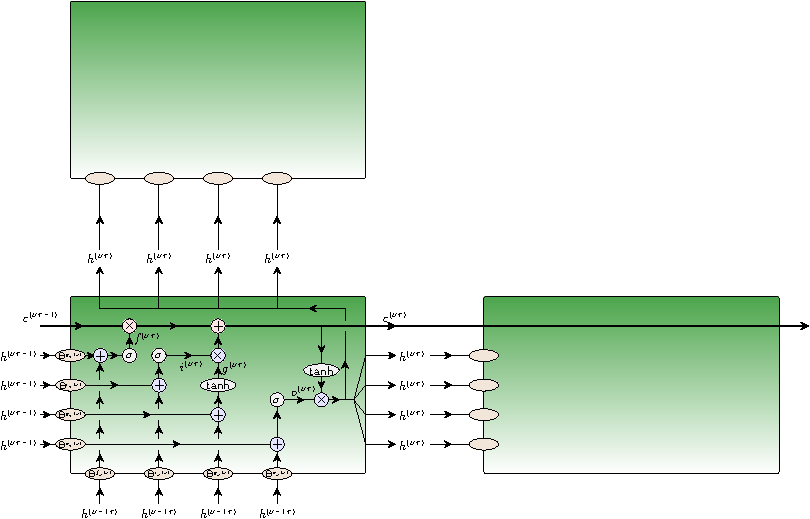
\includegraphics[scale=0.8]{LSTM_structure-tot}};
\end{tikzpicture}
\caption{\label{fig:Lstmall}How the LSTM hidden unit interact with each others}
\end{center}
\end{figure}


\subsection{Forward pass in LSTM}

Considering all the $\tau-1$ variable values to be $0$ when $\tau=0$, we get the following formula for the input, forget and output gates

\begin{align}
i^{(t)(\nu\tau)}_f&=\sigma\left(\sum_{f'=0}^{F_{{\nu-1}}-1}\Theta^{i_{_\nu}(\nu)f}_{f'}
%
h^{(t)(\nu-1\tau)}_{f'}+\sum_{f'=0}^{F{_{\nu}}-1}\Theta^{i_{_\tau}(\nu)f}_{f'}
%
h^{(t)(\nu\tau-1)}_{f'}\right)\;,\\
%
f^{(t)(\nu\tau)}_f&=\sigma\left(\sum_{f'=0}^{F{_{\nu-1}}-1}\Theta^{f_{_\nu}(\nu)f}_{f'}
%
h^{(t)(\nu-1\tau)}_{f'}+\sum_{f'=0}^{F_{{\nu}}-1}\Theta^{f_{_\tau}(\nu)f}_{f'}
%
h^{(t)(\nu\tau-1)}_{f'}\right)\;,\\
%
o^{(t)(\nu\tau)}_f&=\sigma\left(\sum_{f'=0}^{F_{{\nu-1}}-1}\Theta^{o_{_\nu}(\nu)f}_{f'}
%
h^{(t)(\nu-1\tau)}_{f'}+\sum_{f'=0}^{F_{{\nu}}-1}\Theta^{o_{_\tau}(\nu)f}_{f'}
%
h^{(t)(\nu\tau-1)}_{f'}\right)\;.
\end{align}
The sigmoid function is the reason why the $i,f,o$ functions are called gates: they take their values between $0$ and $1$, therefore either allowing or forbidding information to pass through the next step. The cell state update is then performed in the following way
\begin{align}
g^{(t)(\nu\tau)}_f&=\tanh\left(\sum_{f'=0}^{F_{{\nu-1}}-1}\Theta^{g_{_\nu}(\nu)f}_{f'}
%
h^{(t)(\nu-1\tau)}_{f'}+\sum_{f'=0}^{F_{{\nu}}-1}\Theta^{g_{_\tau}(\nu)f}_{f'}
%
h^{(t)(\nu\tau-1)}_{f'}\right)\;,\\
%
c^{(t)(\nu\tau)}_{f}&=
%
f^{(t)(\nu\tau)}_{f}c^{(t)(\nu\tau-1)}_{f}+i^{(t)(\nu\tau)}_{f}g^{(t)(\nu\tau)}_{f}\;,
\end{align}
and as announced, hidden state update is just a probe of the current cell state
\begin{align}
h^{(t)(\nu\tau)}_{f}&=o^{(t)(\nu\tau)}_{f}\tanh \left(c^{(t)(\nu\tau)}_{f}\right)\;.
\end{align}

These formula singularly complicates the feed forward and especially the backpropagation procedure. For completeness, we will us nevertheless carefully derive it. Let us mention in passing that recent studies tried to replace the $\tanh$ activation function of the hidden state $h^{(t)(\nu\tau)}_{f}$ and the cell update $g^{(t)(\nu\tau)}_f$ by Rectified Linear Units, and seems to report better results with a proper initialization of all the weight matrices, argued to be diagonal
\begin{align}
\Theta^f_{f'}(\text{init})&=\frac12\delta^f_{f'}\left(+\sqrt{\frac{6}{F_{\rm in}+F_{\rm out}}}\right)\;,
\end{align}
with the bracket term here to possibly (or not) include some randomness into the initialization

\subsection{Batch normalization}

In batchnorm The update rules for the gates are modified as expected

\begin{align}
i^{(t)(\nu\tau)}_f&=\sigma\left(\sum_{f'=0}^{F_{{\nu-1}}-1}\Theta^{i_\nu(\nu-)f}_{f'}
%
y^{(t)(\nu-1\tau)}_{f'}+\sum_{f'=0}^{F{_{\nu}}-1}\Theta^{i_\tau(-\nu)f}_{f'}
%
y^{(t)(\nu\tau-1)}_{f'}\right)\;,\\
%
f^{(t)(\nu\tau)}_f&=\sigma\left(\sum_{f'=0}^{F{_{\nu-1}}-1}\Theta^{f_\nu(\nu-)f}_{f'}
%
y^{(t)(\nu-1\tau)}_{f'}+\sum_{f'=0}^{F_{{\nu}}-1}\Theta^{f_\tau(-\nu)f}_{f'}
%
y^{(t)(\nu\tau-1)}_{f'}\right)\;,\\
%
o^{(t)(\nu\tau)}_f&=\sigma\left(\sum_{f'=0}^{F_{{\nu-1}}-1}\Theta^{o_\nu(\nu-)f}_{f'}
%
y^{(t)(\nu-1\tau)}_{f'}+\sum_{f'=0}^{F_{{\nu}}-1}\Theta^{o_\tau(-\nu)f}_{f'}
%
y^{(t)(\nu\tau-1)}_{f'}\right)\;,\\
%
g^{(t)(\nu\tau)}_f&=\tanh\left(\sum_{f'=0}^{F_{{\nu-1}}-1}\Theta^{g_\nu(\nu-)f}_{f'}
%
y^{(t)(\nu-1\tau)}_{f'}+\sum_{f'=0}^{F_{{\nu}}-1}\Theta^{g_\tau(-\nu)f}_{f'}
%
y^{(t)(\nu\tau-1)}_{f'}\right)\;,
\end{align}
where
\begin{align}
y^{(t)(\nu\tau)}_{f}&=\gamma^{(\nu\tau)}_{f}\tilde{h}^{(t)(\nu\tau)}_{f}+\beta^{(\nu\tau)}_{f}\;,
\end{align}
as well as
\begin{align}
\tilde{h}^{(t)(\nu\tau)}_{f}&=\frac{h^{(t)(\nu\tau)}_{f}-
%
\hat{h}^{(\nu\tau)}_{f}}{\sqrt{\left(\sigma^{(\nu\tau)}_{f}\right)^2+\epsilon}}
\end{align}
and
\begin{align}
\hat{h}^{(\nu\tau)}_{f}&=\frac{1}{T_{{\rm mb}}}\sum_{t=0}^{T_{{\rm mb}}-1}h^{(t)(\nu\tau)}_{f}\;,&
%
\left(\sigma^{(\nu\tau)}_{f}\right)^2&=\frac{1}{T_{{\rm mb}}}\sum_{t=0}^{T_{{\rm mb}}-1}\left(h^{(t)(\nu\tau)}_{f}
%
-\hat{h}^{(\nu\tau)}_{f}\right)^2\;.
\end{align}
It is important to compute a running sum for the mean and the variance, that will serve for the evaluation of the cross-validation and the test set (calling $e$ the number of iterations/epochs) 
\begin{align}
\mathbb{E}\left[h_{f}^{(t)(\nu\tau)}\right]_{e+1} &=
%
\frac{e\mathbb{E}\left[h_{f}^{(t)(\nu\tau)}\right]_{e}+\hat{h}_{f}^{(\nu\tau)}}{e+1}\;,\\
%
\mathbb{V}ar\left[h_{f}^{(t)(\nu\tau)}\right]_{e+1} &=
%
\frac{e\mathbb{V}ar\left[h_{f}^{(t)(\nu\tau)}\right]_{e}+\left(\hat{\sigma}_{f}^{(\nu\tau)}\right)^2}{e+1}
\end{align}
and what will be used at the end is $\mathbb{E}\left[h_{f}^{(t)(\nu\tau)}\right]$ and $\frac{T_{{\rm mb}}}{T_{{\rm mb}}-1}\mathbb{V}ar\left[h_{f}^{(t)(\nu\tau)}\right]$.



\subsection{Backpropagation in a LSTM} \label{sec:appendbackproplstm}


The backpropagation in a LSTM keeps the same structure as in a RNN, namely 

\begin{align}
\delta^{(t)(N-1\tau)}_f&= \frac{1}{T_{{\rm mb}}}\left(h_{f}^{(t)(N\tau)}-y_f^{(t)(\tau)}\right)\;,
\end{align}
and (shown in appendix \ref{sec:ARNNLSTMerror_rates})
\begin{align}
\delta^{(t)(\nu-1\tau)}_f&= 
%
\sum_{t'=0}^{T_{{\rm mb}}}J^{(tt')(\nu\tau)}_f\sum_{\epsilon=0}^{1}\sum_{f'=0}^{F_{\nu+1-\epsilon}-1}
%
\mathcal{H}^{(t')(\nu-\epsilon\tau+\epsilon)_{b_\epsilon}}_{ff'}\delta^{(t')(\nu-\epsilon\tau+\epsilon)}_{f'}\;.
\end{align}
What changes is the form of $\mathcal{H}$, now given by
\begin{align}
\mathcal{O}^{(t)(\nu\tau)}_{f}&=h^{(t)(\nu\tau)}_{f}
%
\left(1-o^{(t)(\nu\tau)}_{f}\right)\;,\notag\\
%
\mathcal{I}^{(t)(\nu\tau)}_{f}&=o^{(t)(\nu\tau)}_{f}\left(1-\tanh^2\left(c^{(t)(\nu\tau)}_{f}\right)
%
\right)g^{(t)(\nu\tau)}_{f} i^{(t)(\nu\tau)}_{f}\left(1-i^{(t)(\nu\tau)}_{f}\right)\;,\notag\\
%
\mathcal{F}^{(t)(\nu\tau)}_{f}&=o^{(t)(\nu\tau)}_{f}\left(1-\tanh^2\left(c^{(t)(\nu\tau)}_{f}\right)
%
\right)c^{(t)(\nu\tau-1)}_{f} f^{(t)(\nu\tau)}_{f}\left(1-f^{(t)(\nu\tau)}_{f}\right)\;,\notag\\
%
\mathcal{G}^{(t)(\nu\tau)}_{f}&=o^{(t)(\nu\tau)}_{f}\left(1-\tanh^2\left(c^{(t)(\nu\tau)}_{f}\right)
%
\right)i^{(t)(\nu\tau)}_{f}\left(1-\left(g^{(t)(\nu\tau)}_{f}\right)^2\right)\;,
\end{align}

and

\begin{align}
H^{(t)(\nu\tau)_a}_{ff'}&=\Theta^{o_a(\nu+1)f'}_{f}\mathcal{O}^{(t)(\nu+1\tau)}_{f'}
%
+\Theta^{f_a(\nu+1)f'}_{f}\mathcal{F}^{(t)(\nu+1\tau)}_{f'}\notag\\
%
&+\Theta^{g_a(\nu+1)f'}_{f}\mathcal{G}^{(t)(\nu+1\tau)}_{f'}
%
+\Theta^{i_a(\nu+1)f'}_{f}\mathcal{I}^{(t)(\nu+1\tau)}_{f'}\;.
\end{align}


\subsection{Weight and coefficient updates in a LSTM}

As for the RNN, (but with the $\mathcal{H}$ defined in section \ref{sec:appendbackproplstm}), we get for $\nu=1$
\begin{align}
\Delta^{\rho_\nu(\nu)f}_{f'}&=\sum_{\tau=0}^{T-1}\sum_{t=0}^{T_{{\rm mb}}-1}
%
\rho^{(\nu\tau)(t)}_{f}\delta^{(\nu\tau)(t)}_{f}h^{(\nu-1\tau)(t)}_{f'}\;,\\
\end{align}
and otherwise
\begin{align}
\Delta^{\rho_\nu(\nu)f}_{f'}&=\sum_{\tau=0}^{T-1}\sum_{t=0}^{T_{{\rm mb}}-1}
%
\rho^{(\nu\tau)(t)}_{f}\delta^{(\nu\tau)(t)}_{f}y^{(\nu-1\tau)(t)}_{f'}\;,\\
%
\rho^{(\nu\tau)(t)}_{f}\delta^{(\nu\tau)(t)}_{f}y^{(\nu-1\tau)(t)}_{f'}\;,\\
%
\Delta^{\rho_\tau(\nu)f}_{f'}&=\sum_{\tau=1}^{T-1}\sum_{t=0}^{T_{{\rm mb}}-1}
%
\rho^{(\nu\tau)(t)}_{f}\delta^{(\nu\tau)(t)}_{f}y^{(\nu\tau-1)(t)}_{f'}\;,\\
%
\Delta^{\beta(\nu \tau)}_{f}&=\sum_{t=0}^{T_{{\rm mb}}-1}\sum_{\epsilon=0}^{1}\sum_{f'=0}^{F_{\nu+1-\epsilon}-1}
%
\mathcal{H}^{(t)(\nu-\epsilon\tau+\epsilon)_{b_\epsilon}}_{ff'}\delta^{(t)(\nu-\epsilon\tau+\epsilon)}_{f'}\;,\\
%
\Delta^{\gamma(\nu \tau)}_{f}&=\sum_{t=0}^{T_{{\rm mb}}-1}\tilde{h}^{(t)(\nu\tau)}_{f}\sum_{\epsilon=0}^{1}\sum_{f'=0}^{F_{\nu+1-\epsilon}-1}
%
\mathcal{H}^{(t)(\nu-\epsilon\tau+\epsilon)_{b_\epsilon}}_{ff'}\delta^{(t)(\nu-\epsilon\tau+\epsilon)}_{f'}\;.
\end{align}

and

\begin{align}
\Delta^{f}_{f'}&=\sum_{\tau=0}^{T-1}\sum_{t=0}^{T_{{\rm mb}}-1} y^{(t)(N-1\tau)}_{f'}\delta^{(t)(N-1\tau)}_{f}\;.
\end{align}


\begin{subappendices}


\section{Backpropagation trough Batch Normalization}

For Backpropagation, we will need 

\begin{align}
\frac{\partial y^{(t')(\nu\tau)}_{f'}}{\partial h_{f}^{(t)(\nu\tau)}}&=
%
\gamma^{(\nu\tau)}_f\frac{\partial \tilde{h}_{f'}^{(t)(\nu\tau)}}{\partial h_{f}^{(t)(\nu\tau)}}\;.
\end{align}

Since

\begin{align}
\frac{\partial h^{(t')(\nu\tau)}_{f'}}{\partial h_{f}^{(t)(\nu\tau)}}&=\delta^{t'}_t\delta^{f'}_f\;,&
%
\frac{\partial \hat{h}_{f'}^{(\nu\tau)}}{\partial h_{f}^{(t)(\nu\tau)}}&=\frac{\delta^{f'}_f}{T_{{\rm mb}}}\:;
\end{align}

and

\begin{align}
\frac{\partial \left(\hat{\sigma}_{f'}^{(\nu\tau)}\right)^2}{\partial h_{f}^{(t)(\nu\tau)}}&=
%
\frac{2\delta^{f'}_f}{T_{{\rm mb}}}\left(h_{f}^{(t)(\nu\tau)}-\hat{h}_{f}^{(\nu\tau)}\right)\;,
\end{align}

we get

\begin{align}
\frac{\partial \tilde{h}_{f'}^{(t')(\nu\tau)}}{\partial h_{f}^{(t)(\nu\tau)}}&=
%
\frac{\delta^{f'}_f}{T_{{\rm mb}}}\left[\frac{T_{{\rm mb}}\delta^{t'}_t-1}
%
{\left(\left(\hat{\sigma}_{f}^{(\nu\tau)}\right)^2+\epsilon\right)^\frac12}-
%
\frac{\left(h_{f}^{(t')(\nu\tau)}-\hat{h}_{f}^{(\nu\tau)}\right)\left(h_{f}^{(t)(\nu\tau)}-\hat{h}_{f}^{(\nu\tau)}\right)}
%
{\left(\left(\hat{\sigma}_{f}^{(\nu\tau)}\right)^2+\epsilon\right)^\frac32}\right]\notag\\
%
&=\frac{\delta^{f'}_f}{\left(\left(\hat{\sigma}_{f}^{(\nu\tau)}\right)^2+\epsilon\right)^\frac12}
%
\left[\delta^{t'}_t-
%
\frac{1+\tilde{h}_{f}^{(t')(\nu\tau)}\tilde{h}_{f}^{(t)(\nu\tau)}}{T_{{\rm mb}}}\right]\;.
\end{align}

To ease the notation we will denote

\begin{align}
\tilde{\gamma}^{(\nu\tau)}_f&=
%
\frac{\gamma^{(\nu\tau)}_f}{\left(\left(\hat{\sigma}_{f}^{(\nu\tau)}\right)^2+\epsilon\right)^\frac12}\;.
\end{align}

so that

\begin{align}
\frac{\partial y_{f'}^{(t')(\nu\tau)}}{\partial h_{f}^{(t)(\nu\tau)}}&=
%
\tilde{\gamma}^{(\nu\tau)}_f \delta^{f'}_f\left[\delta^{t'}_t-
%
\frac{1+\tilde{h}_{f}^{(t')(\nu\tau)}\tilde{h}_{f}^{(t)(\nu\tau)}}{T_{{\rm mb}}}\right]\;.
\end{align}

This modifies the error rate backpropagation, as well as the formula for the weight update ($y$'s instead of $h$'s). In the following we will use the formula

\begin{align}
J^{(tt')(\nu\tau)}_{f}&=
%
\tilde{\gamma}^{(\nu\tau)}_f \left[\delta^{t'}_t-
%
\frac{1+\tilde{h}_{f}^{(t')(\nu\tau)}\tilde{h}_{f}^{(t)(\nu\tau)}}{T_{{\rm mb}}}\right]\;.
\end{align}


\section{RNN Backpropagation}

\subsection{RNN Error rate updates: details} \label{sec:rnnappenderrorrate}

Recalling the error rate definition

\begin{align}
\delta^{(t)( \nu\tau)}_f&=\frac{\delta}{\delta h^{(t)( \nu+1\tau)}_f }J(\Theta)\;,
\end{align}

we would like to compute it for all existing values of $\nu$ and $\tau$. As computed in chapter \ref{sec:chapterFNN}, one has for the maximum $\nu$ value

\begin{align}
\delta^{(t)(N-1\tau)}_f&= \frac{1}{T_{{\rm mb}}}\left(h_{f}^{(t)(N\tau)}-y_f^{(t)(\tau)}\right)\;.
\end{align}

Now since (taking Batch Normalization into account)

\begin{align}
h^{(t)(N\tau)}_{f}&=o\left(\sum_{f'=0}^{F_{N-1}-1}\Theta^f_{f'} y^{(t)(N-1\tau)}_{f}\right)\;,
\end{align}

and 

\begin{align}
h^{(t)(\nu\tau)}_f&=\tanh\left(\sum_{f'=0}^{F_{{\nu-1}}-1}\Theta^{\nu(\nu)f}_{f'}
%
y^{(t)(\nu-1\tau)}_{f'}+\sum_{f'=0}^{F_{{\nu}}-1}\Theta^{\tau(\nu)f}_{f'}
%
y^{(t)(\nu\tau-1)}_{f'}\right)\;,
\end{align}

we get for 

\begin{align}
\delta^{(t)(N-2\tau)}_f&= \sum_{t'=0}^{T_{{\rm mb}}}\left[\sum_{f'=0}^{F_{N}-1}
%
\frac{\delta h^{(t')(N\tau)}_{f'}}{\delta h^{(t)(N-1\tau)}_f }\delta^{(t')(N-1\tau)}_{f'}\right.\notag\\
%
&+\left.\sum_{f'=0}^{F_{N-1}-1}\frac{\delta h^{(t')(N-1\tau+1)}_{f'}}{\delta h^{(t)(N-1\tau)}_f }\delta^{(t')(N-2\tau+1)}_{f'}\right]\;.
\end{align}

Let us work out explicitly once (for a regression cost function and a trivial identity output function)

\begin{align}
\frac{\delta h^{(t')(N\tau)}_{f'}}{\delta h^{(t)(N-1\tau)}_f }&=\sum_{f''=0}^{F_{N-1}-1}\Theta^{f'}_{f''}\,
%
\frac{\delta y^{(t')(N-1\tau)}_{f''}}{\delta h^{(t)(N-1\tau)}_f } \notag\\
%
&=\Theta^{f'}_{f}\,J_f^{(tt')(N-1\tau)}\;.
\end{align}

as well as

\begin{align}
\frac{\delta h^{(t')(N-1\tau+1)}_{f'}}{\delta h^{(t)(N-1\tau)}_f }&=
%
\left[1-\left(h^{(t')(N-1\tau+1)}_{f'}\right)^2\right]\sum_{f''=0}^{F_{{N-1}}-1}\Theta^{\tau(N-1)f'}_{f''}
%
\frac{\delta y^{(t')(N-1\tau)}_{f''}}{\delta h^{(t)(N-1\tau)}_f }\notag\\
%
&=\mathcal{T}^{(t')(N-1\tau+1)}_{f'}\Theta^{\tau(N-1)f'}_{f}\,J_f^{(tt')(N-1\tau)}\;.
\end{align}

Thus

\begin{align}
\delta^{(t)(N-2\tau)}_f&= \sum_{t'=0}^{T_{{\rm mb}}}J_f^{(tt')(N-1\tau)}\left[\sum_{f'=0}^{F_{N}-1}
%
\Theta^{f'}_{f}\,\delta^{(t')(N-1\tau)}_{f'}\right.\notag\\
%
&\left.+\sum_{f'=0}^{F_{N-1}-1}\mathcal{T}^{(t')(N-1\tau+1)}_{f'}\Theta^{\tau(N-1)f'}_{f}\,\delta^{(t')(N-2\tau+1)}_{f'}\right]\;.
\end{align}

Here we adopted the convention that the $\delta^{(t')(N-2\tau+1)}$'s are $0$ if $\tau=T$. In a similar way, we derive for $\nu\leq N-1$

\begin{align}
\delta^{(t)(\nu-1\tau)}_f&= \sum_{t'=0}^{T_{{\rm mb}}}J^{(tt')(\nu\tau)}_f\left[\sum_{f'=0}^{F_{\nu+1}-1}
%
\mathcal{T}^{(t')(\nu+1\tau)}_{f'}\Theta^{\nu(\nu+1)f'}_{f}\,\delta^{(t')(\nu\tau)}_{f'}\right.\notag\\
%
&\left.+\sum_{f'=0}^{F_{\nu}-1}\mathcal{T}^{(t')(\nu\tau+1)}_{f'}\Theta^{\tau(\nu)f'}_{f}\,\delta^{(t')(\nu-1\tau+1)}_{f'}\right]\;.
\end{align}

Defining 

\begin{align}
\mathcal{T}^{(t')(N\tau)}_{f'}&=1\;,&
%
\Theta^{\nu(N)f'}_{f}&=\Theta^{f'}_{f}\;,
\end{align}

the previous $ \delta^{(t)(\nu-1\tau)}_f$ formula extends to the case $\nu  =N-1$. To unite the RNN and the LSTM formulas, let us finally define (with $a$ either $\tau$ or $\nu$

\begin{align}
\mathcal{H}^{(t')(\nu\tau)_a}_{ff'}&=\mathcal{T}^{(t')(\nu+1\tau)}_{f'}\Theta^{a(\nu+1)f'}_{f}\;,
\end{align}

thus (defining $b_0=\nu$ and $b_1=\tau$)

\begin{align}
\delta^{(t)(\nu-1\tau)}_f&= 
%
\sum_{t'=0}^{T_{{\rm mb}}}J^{(tt')(\nu\tau)}_f\sum_{\epsilon=0}^{1}\sum_{f'=0}^{F_{\nu+1-\epsilon}-1}
%
\mathcal{H}^{(t')(\nu-\epsilon\tau+\epsilon)_{b_\epsilon}}_{ff'}\delta^{(t')(\nu-\epsilon\tau+\epsilon)}_{f'}\;.
\end{align}


\subsection{RNN Weight and coefficient updates: details} \label{sec:rnncoefficient}

We want here to derive 

\begin{align}
\Delta^{\nu(\nu)f}_{f'}&=\frac{\partial}{\partial \Theta^{\nu(\nu)f}_{f'}} J(\Theta)&
%
\Delta^{\tau(\nu)f}_{f'}&=\frac{\partial}{\partial \Theta^{\tau(\nu)f}_{f'}} J(\Theta)\;.
\end{align}

We first expand

\begin{align}
\Delta^{\nu(\nu)f}_{f'}&=\sum_{\tau=0}^{T-1}\sum_{f''=0}^{F_\nu-1}\sum_{t=0}^{T_{{\rm mb}}-1}
%
\frac{\partial h^{(t)(\nu\tau)}_{f''}}{\partial \Theta^{\nu(\nu)f}_{f'}}
%
\delta^{(t)(\nu-1\tau)}_{f''}\;,\notag\\
%
\Delta^{\tau(\nu)f}_{f'}&=\sum_{\tau=0}^{T-1}\sum_{f''=0}^{F_\nu-1}\sum_{t=0}^{T_{{\rm mb}}-1}
%
\frac{\partial h^{(t)(\nu\tau)}_{f''}}{\partial \Theta^{\tau(\nu)f}_{f'}}
%
\delta^{(t)(\nu-1\tau)}_{f''}\;,
\end{align}

so that

\begin{align}
\Delta^{\nu(\nu)f}_{f'}&=\sum_{\tau=0}^{T-1}\sum_{t=0}^{T_{{\rm mb}}-1}
%
\mathcal{T}^{(t)(\nu\tau)}_{f}\delta^{(t)(\nu-1\tau)}_{f}h^{(t)(\nu-1\tau)}_{f'}\;,\\
%
\Delta^{\tau(\nu)f}_{f'}&=\sum_{\tau=1}^{T-1}\sum_{t=0}^{T_{{\rm mb}}-1}
%
\mathcal{T}^{(t)(\nu\tau)}_{f}\delta^{(t)(\nu-1\tau)}_{f}h^{(t)(\nu\tau-1)}_{f'}\;.
\end{align}

We also have to compute

\begin{align}
\Delta^{f}_{f'}&=\frac{\partial}{\partial \Theta^{f}_{f'}} J(\Theta)\;.
\end{align}

We first expand

\begin{align}
\Delta^{f}_{f'}&=\sum_{\tau=0}^{T-1}\sum_{f''=0}^{F_N-1}\sum_{t=0}^{T_{{\rm mb}}-1}
%
\frac{\partial h^{(t)(N\tau)}_{f''}}{\partial \Theta^{f}_{f'}}
%
\delta^{(t)(N-1\tau)}_{f''}\;
\end{align}

so that

\begin{align}
\Delta^{f}_{f'}&=\sum_{\tau=0}^{T-1}\sum_{t=0}^{T_{{\rm mb}}-1} h^{(t)(N-1\tau)}_{f'}\delta^{(t)(N-1\tau)}_{f}\;.
\end{align}

Finally, we need

\begin{align}
\Delta^{\beta(\nu \tau)}_{f}&=\frac{\partial}{\partial\beta^{(\nu \tau)}_{f}} J(\Theta)&
%
\Delta^{\gamma(\nu \tau)}_{f}&=\frac{\partial}{\partial \gamma^{(\nu \tau)}_{f}} J(\Theta)\;.
\end{align}

First

\begin{align}
\Delta^{\beta(\nu \tau)}_{f}&=\sum_{t=0}^{T_{{\rm mb}}-1}\left[\sum_{f'=0}^{F_{\nu+1}-1}
%
\frac{\partial h^{(t)(\nu+1\tau)}_{f'}}{\partial \beta^{(\nu \tau)}_{f}}\delta^{(t)(\nu\tau)}_{f'}+
%
\sum_{f'=0}^{F_{\nu}-1}
%
\frac{\partial h^{(t)(\nu\tau+1)}_{f'}}{\partial \beta^{(\nu \tau)}_{f}}\delta^{(t)(\nu-1\tau+1)}_{f'}\right]\;,\notag\\
%
\Delta^{\gamma(\nu \tau)}_{f}&=\sum_{t=0}^{T_{{\rm mb}}-1}\left[\sum_{f'=0}^{F_{\nu+1}-1}
%
\frac{\partial h^{(t)(\nu+1\tau)}_{f'}}{\partial \gamma^{(\nu \tau)}_{f}}\delta^{(t)(\nu\tau)}_{f'}+
%
\sum_{f'=0}^{F_{\nu}-1}
%
\frac{\partial h^{(t)(\nu\tau+1)}_{f'}}{\partial \gamma^{(\nu \tau)}_{f}}\delta^{(t)(\nu-1\tau+1)}_{f'}\right]\;.
\end{align}

So that

\begin{align}
\Delta^{\beta(\nu \tau)}_{f}&=\sum_{t=0}^{T_{{\rm mb}}-1}\left[\sum_{f'=0}^{F_{\nu+1}-1}
%
\mathcal{T}^{(t)(\nu+1\tau)}_{f'}\Theta^{\nu(\nu+1)f'}_{f}\delta^{(t)(\nu\tau)}_{f'}\right.\notag\\
%
&\left.+\sum_{f'=0}^{F_{\nu}-1}
%
\mathcal{T}^{(t)(\nu\tau+1)}_{f'}\Theta^{\tau(\nu)f'}_{f}\delta^{(t)(\nu-1\tau+1)}_{f'}\right]\;,\\
%
\Delta^{\gamma(\nu \tau)}_{f}&=\sum_{t=0}^{T_{{\rm mb}}-1}\left[\sum_{f'=0}^{F_{\nu+1}-1}
%
\mathcal{T}^{(t)(\nu+1\tau)}_{f'}\Theta^{\nu(\nu+1)f'}_{f}
%
\tilde{h}^{(t)(\nu\tau)}_{f}\delta^{(t)(\nu\tau)}_{f'}\right.\notag\\
%
&\left.+\sum_{f'=0}^{F_{\nu}-1}\mathcal{T}^{(t)(\nu\tau+1)}_{f'}
%
\Theta^{\tau(\nu)f'}_{f}\tilde{h}^{(t)(\nu\tau)}_{f}\delta^{(t)(\nu-1\tau+1)}_{f'}\right]\;,
\end{align}

which we can rewrite as

\begin{align}
\Delta^{\beta(\nu \tau)}_{f}&=\sum_{t=0}^{T_{{\rm mb}}-1}\sum_{\epsilon=0}^{1}\sum_{f'=0}^{F_{\nu+1-\epsilon}-1}
%
\mathcal{H}^{(t)(\nu-\epsilon\tau+\epsilon)_{b_\epsilon}}_{ff'}\delta^{(t)(\nu-\epsilon\tau+\epsilon)}_{f'}\;,\\
%
\Delta^{\gamma(\nu \tau)}_{f}&=\sum_{t=0}^{T_{{\rm mb}}-1}\tilde{h}^{(t)(\nu\tau)}_{f}\sum_{\epsilon=0}^{1}\sum_{f'=0}^{F_{\nu+1-\epsilon}-1}
%
\mathcal{H}^{(t)(\nu-\epsilon\tau+\epsilon)_{b_\epsilon}}_{ff'}\delta^{(t)(\nu-\epsilon\tau+\epsilon)}_{f'}\;.
\end{align}

\section{LSTM Backpropagation}




\subsection{LSTM Error rate updates: details} \label{sec:ARNNLSTMerror_rates}

As for the RNN 

\begin{align}
\delta^{(t)(N-1\tau)}_{f}&
%
=\frac{1}{T_{{\rm mb}}}\left(h^{(t)(N\tau)}_{f}-y^{(t)(\tau)}_{f}\right)\;.
\end{align}

Before  going any further, it will be useful to define 

\begin{align}
\mathcal{O}^{(t)(\nu\tau)}_{f}&=h^{(t)(\nu\tau)}_{f}
%
\left(1-o^{(t)(\nu\tau)}_{f}\right)\;,\notag\\
%
\mathcal{I}^{(t)(\nu\tau)}_{f}&=o^{(t)(\nu\tau)}_{f}\left(1-\tanh^2\left(c^{(t)(\nu\tau)}_{f}\right)
%
\right)g^{(t)(\nu\tau)}_{f} i^{(t)(\nu\tau)}_{f}\left(1-i^{(t)(\nu\tau)}_{f}\right)\;,\notag\\
%
\mathcal{F}^{(t)(\nu\tau)}_{f}&=o^{(t)(\nu\tau)}_{f}\left(1-\tanh^2\left(c^{(t)(\nu\tau)}_{f}\right)
%
\right)c^{(t)(\nu\tau-1)}_{f} f^{(t)(\nu\tau)}_{f}\left(1-f^{(t)(\nu\tau)}_{f}\right)\;,\notag\\
%
\mathcal{G}^{(t)(\nu\tau)}_{f}&=o^{(t)(\nu\tau)}_{f}\left(1-\tanh^2\left(c^{(t)(\nu\tau)}_{f}\right)
%
\right)i^{(t)(\nu\tau)}_{f}\left(1-\left(g^{(t)(\nu\tau)}_{f}\right)^2\right)\;,
\end{align}

and

\begin{align}
H^{(t)(\nu\tau)_a}_{ff'}&=\Theta^{o_a(\nu+1)f'}_{f}\mathcal{O}^{(t)(\nu+1\tau)}_{f'}
%
+\Theta^{f_a(\nu+1)f'}_{f}\mathcal{F}^{(t)(\nu+1\tau)}_{f'}\notag\\
%
&+\Theta^{g_a(\nu+1)f'}_{f}\mathcal{G}^{(t)(\nu+1\tau)}_{f'}
%
+\Theta^{i_a(\nu+1)f'}_{f}\mathcal{I}^{(t)(\nu+1\tau)}_{f'}\;.
\end{align}

As for RNN, we will start off by looking at 

\begin{align}
\delta^{(t)(N-2\tau)}_f&= \sum_{t'=0}^{T_{{\rm mb}}}\left[\sum_{f'=0}^{F_{N}-1}
%
\frac{\delta h^{(t')(N\tau)}_{f'}}{\delta h^{(t)(N-1\tau)}_f }\delta^{(t')(N-1\tau)}_{f'}\right.\notag\\
%
&+\left.\sum_{f'=0}^{F_{N-1}-1}\frac{\delta h^{(t')(N-1\tau+1)}_{f'}}{\delta h^{(t)(N-1\tau)}_f }\delta^{(t')(N-2\tau+1)}_{f'}\right]\;.
\end{align}

We will be able to get our hands on the second term with the general formula, so let us first look at

\begin{align}
\frac{\delta h^{(t')(N\tau)}_{f'}}{\delta h^{(t)(N-1\tau)}_f }&=\Theta^{f'}_{f}\,J_f^{(tt')(N-1\tau)}\;,
\end{align}

which is is similar to the RNN case. Let us put aside the second term of $\delta^{(t)(N-2\tau)}_f$, and look at the general case

\begin{align}
\delta^{(t)(\nu-1\tau)}_f&= \sum_{t'=0}^{T_{{\rm mb}}}\left[\sum_{f'=0}^{F_{\nu+1}-1}
%
\frac{\delta h^{(t')(\nu+1\tau)}_{f'}}{\delta h^{(t)(\nu\tau)}_f }\delta^{(t')(\nu\tau)}_{f'}
%
+\sum_{f'=0}^{F_{\nu}-1}\frac{\delta h^{(t')(\nu\tau+1)}_{f'}}{\delta h^{(t)(\nu\tau)}_f }\delta^{(t')(\nu-1\tau+1)}_{f'}\right]\;,
\end{align}
which involves to study in details
\begin{align}
\frac{\delta h^{(t')(\nu+1\tau)}_{f'}}{\delta h^{(t)(\nu\tau)}_f }&=
%
\frac{\delta o^{(t')(\nu+1\tau)}_{f'}}{\delta h^{(t)(\nu\tau)}_f }\tanh  c^{(t')(\nu+1\tau)}_{f'}\notag\\
%
&+\frac{\delta c^{(t')(\nu+1\tau)}_{f'}}{\delta h^{(t)(\nu\tau)}_f } o^{(t')(\nu+1\tau)}_{f'}
%
\left[1-\tanh^2  c^{(t')(\nu+1\tau)}_{f'}\right]\;.
\end{align}
Now
\begin{align}
\frac{\delta o^{(t')(\nu+1\tau)}_{f'}}{\delta h^{(t)(\nu\tau)}_f }&=o^{(t')(\nu+1\tau)}_{f'}
%
\left[1-o^{(t')(\nu+1\tau)}_{f'}\right]\sum_{f''=0}^{F_\nu-1}\Theta^{o_\nu(\nu+1)f'}_{f''}
%
\frac{\delta y^{(t')(\nu\tau)}_{f'}}{\delta h^{(t)(\nu\tau)}_f }\notag\\
%
&=o^{(t')(\nu+1\tau)}_{f'}
%
\left[1-o^{(t')(\nu+1\tau)}_{f'}\right]\Theta^{o_\nu(\nu+1)f'}_{f}
%
J^{(tt')(\nu\tau)}_f\;,
\end{align}
and
\begin{align}
\frac{\delta c^{(t')(\nu+1\tau)}_{f'}}{\delta h^{(t)(\nu\tau)}_f }&=
%
\frac{\delta i^{(t')(\nu+1\tau)}_{f'}}{\delta h^{(t)(\nu\tau)}_f }g^{(t')(\nu+1\tau)}_{f'}
%
+\frac{\delta g^{(t')(\nu+1\tau)}_{f'}}{\delta h^{(t)(\nu\tau)}_f }i^{(t')(\nu+1\tau)}_{f'}\notag\\
%
&+\frac{\delta f^{(t')(\nu+1\tau)}_{f'}}{\delta h^{(t)(\nu\tau)}_f }c^{(t')(\nu\tau)}_{f'}\;.
\end{align}
We continue our journey
\begin{align}
\frac{\delta i^{(t')(\nu+1\tau)}_{f'}}{\delta h^{(t)(\nu\tau)}_f }&=
%
 i^{(t')(\nu+1\tau)}_{f'}\left[1-  i^{(t')(\nu+1\tau)}_{f'}\right]\Theta^{i_\nu(\nu+1)f'}_{f}
%
J^{(tt')(\nu\tau)}_f\;,\notag\\
%
\frac{\delta f^{(t')(\nu+1\tau)}_{f'}}{\delta h^{(t)(\nu\tau)}_f }&=
%
 f^{(t')(\nu+1\tau)}_{f'}\left[1-  f^{(t')(\nu+1\tau)}_{f'}\right]\Theta^{f_\nu(\nu+1)f'}_{f}
%
J^{(tt')(\nu\tau)}_f\;,\notag\\
%
\frac{\delta g^{(t')(\nu+1\tau)}_{f'}}{\delta h^{(t)(\nu\tau)}_f }&=
%
\left[1-  \left(g^{(t')(\nu+1\tau)}_{f'}\right)^2\right]\Theta^{g_\nu(\nu+1)f'}_{f}
%
J^{(tt')(\nu\tau)}_f\;,
\end{align}
and our notations now come handy
\begin{align}
\frac{\delta h^{(t')(\nu+1\tau)}_{f'}}{\delta h^{(t)(\nu\tau)}_f }&=J^{(tt')(\nu\tau)}_fH^{(t)(\nu\tau)_\nu}_{ff'}\;.
\end{align}
This formula also allows us to compute the second term for $\delta^{(t)(N-2\tau)}_f$. In a totally similar manner
\begin{align}
\frac{\delta h^{(t')(\nu\tau+1)}_{f'}}{\delta h^{(t)(\nu\tau)}_f }&=J^{(tt')(\nu\tau)}_fH^{(t)(\nu-1\tau+1)_\tau}_{ff'}\;.
\end{align}
Going back to our general formula
\begin{align}
\delta^{(t)(\nu-1\tau)}_f&= \sum_{t'=0}^{T_{{\rm mb}}}J^{(tt')(\nu\tau)}_f\left[\sum_{f'=0}^{F_{\nu+1}-1}
%
H^{(t)(\nu\tau)_\nu}_{ff'}\delta^{(t')(\nu\tau)}_{f'}\right.\notag\\
%
&+\left.\sum_{f'=0}^{F_{\nu}-1}H^{(t)(\nu-1\tau+1)_\tau}_{ff'}\delta^{(t')(\nu-1\tau+1)}_{f'}\right]\;,
\end{align}
and as in the RNN case, we re-express it as (defining $b_0=\nu$ and $b_1=\tau$)
\begin{align}
\delta^{(t)(\nu-1\tau)}_f&= 
%
\sum_{t'=0}^{T_{{\rm mb}}}J^{(tt')(\nu\tau)}_f\sum_{\epsilon=0}^{1}\sum_{f'=0}^{F_{\nu+1-\epsilon}-1}
%
\mathcal{H}^{(t')(\nu-\epsilon\tau+\epsilon)_{b_\epsilon}}_{ff'}\delta^{(t')(\nu-\epsilon\tau+\epsilon)}_{f'}\;.
\end{align}
This formula is also valid for $\nu  =N-1$ if we define as for the RNN case
\begin{align}
\mathcal{H}^{(t')(N\tau)}_{f'}&=1\;,&
%
\Theta^{\nu(N)f'}_{f}&=\Theta^{f'}_{f}\;,
\end{align}
 


\subsection{LSTM Weight and coefficient updates: details}

We want to compute 

\begin{align}
\Delta^{\rho_{_\nu}(\nu)f}_{f'}&=\frac{\partial}{\partial \Theta^{\rho_{_\nu}(\nu)f}_{f'}} J(\Theta)&
%
\Delta^{\rho_{_\tau}(\nu)f}_{f'}&=\frac{\partial}{\partial \Theta^{\rho_{_\tau}(\nu)f}_{f'}} J(\Theta)\;,
\end{align}

with $\rho = (f,i,g,o)$. First we expand

\begin{align}
\Delta^{\rho_{_\nu}(\nu)f}_{f'}&=\sum_{\tau=0}^{T-1}\sum_{f''=0}^{F_\nu-1}\sum_{t=0}^{T_{{\rm mb}}-1}
%
\frac{\partial h^{(\nu\tau)(t)}_{f''}}{\partial \Theta^{\rho_{_\nu}(\nu)f}_{f'}}
%
\frac{\partial}{\partial h^{(\nu\tau)(t)}_{f''}} J(\Theta)\notag\\
%
&=\sum_{\tau=0}^{T-1}\sum_{f''=0}^{F_\nu-1}\sum_{t=0}^{T_{{\rm mb}}-1}
%
\frac{\partial h^{(\nu\tau)(t)}_{f''}}{\partial \Theta^{\rho_{_\nu}(\nu)f}_{f'}}
%
\delta^{(\nu\tau)(t)}_{f''}\;,
\end{align}

so that (with $\rho^{(\nu\tau)}=\left(\mathcal{F},\mathcal{I},\mathcal{G},\mathcal{O}\right)$) if $\nu=1$

\begin{align}
\Delta^{\rho_\nu(\nu-)f}_{f'}&=\sum_{\tau=0}^{T-1}\sum_{t=0}^{T_{{\rm mb}}-1}
%
\rho^{(\nu\tau)(t)}_{f}\delta^{(\nu\tau)(t)}_{f}h^{(\nu-1\tau)(t)}_{f'}\;,
\end{align}

and else

\begin{align}
\Delta^{\rho_\nu(\nu-)f}_{f'}&=\sum_{\tau=0}^{T-1}\sum_{t=0}^{T_{{\rm mb}}-1}
%
\rho^{(\nu\tau)(t)}_{f}\delta^{(\nu\tau)(t)}_{f}y^{(\nu-1\tau)(t)}_{f'}\;,\\
%
\Delta^{\rho_\tau(\nu)f}_{f'}&=\sum_{\tau=1}^{T-1}\sum_{t=0}^{T_{{\rm mb}}-1}
%
\rho^{(\nu\tau)(t)}_{f}\delta^{(\nu\tau)(t)}_{f}y^{(\nu\tau-1)(t)}_{f'}\;.
\end{align}

We will now need to compute

\begin{align}
\Delta^{\beta(\nu\tau)}_{f}&=\frac{\partial}{\partial \beta^{(\nu\tau)}_f} J(\Theta)&
%
\Delta^{\gamma(\nu\tau)}_{f}&=\frac{\partial}{\partial \gamma^{(\nu\tau)}_f} J(\Theta)\;.
\end{align}

For that we need to look at 

\begin{align}
\Delta^{\beta(\nu\tau)}_{f}&=\sum_{f'=0}^{F_{\nu+1}-1}\sum_{t'=0}^{T_{{\rm mb}}-1}
%
\frac{\partial h^{(\nu+1\tau)(t')}_{f'}}{\partial \beta^{(\nu\tau)}_f}\delta^{(\nu\tau)(t')}_{f'}
%
+\sum_{f'=0}^{F_{\nu}-1}\sum_{t'=0}^{T_{{\rm mb}}-1}\frac{\partial h^{(\nu\tau+1)(t')}_{f'}}
%
{\partial \beta^{(\nu\tau)}_f}\delta^{(\nu-1\tau+1)(t')}_{f'}\notag\\
%
&=\sum_{t=0}^{T_{{\rm mb}}-1}\left\{\sum_{f'=0}^{F_{\nu+1}-1}
%
H^{(t)(\nu\tau)}_{ff'}\delta^{(t)(\nu\tau)}_{f'}
%
+\sum_{f'=0}^{F_{\nu}-1}H^{(t)(\nu-1\tau+1)}_{ff'}\delta^{(t)(\nu\tau+1)}_{f'}\right\}\;. 
\end{align}

and

\begin{align}
\Delta^{\gamma(\nu\tau)}_{f}&=\sum_{t=0}^{T_{{\rm mb}}-1}\tilde{h}^{(t)(\nu\tau)}_{f}\left\{\sum_{f'=0}^{F_{\nu+1}-1}
%
H^{(t)(\nu\tau)}_{ff'}\delta^{(t)(\nu\tau)}_{f'}
%
+\sum_{f'=0}^{F_{\nu}-1}H^{(t)(\nu-1\tau+1)}_{ff'}\delta^{(t)(\nu-1\tau+1)}_{f'}\right\}\;,
\end{align}

which we can rewrite as

\begin{align}
\Delta^{\beta(\nu \tau)}_{f}&=\sum_{t=0}^{T_{{\rm mb}}-1}\sum_{\epsilon=0}^{1}\sum_{f'=0}^{F_{\nu+1-\epsilon}-1}
%
\mathcal{H}^{(t)(\nu-\epsilon\tau+\epsilon)_{b_\epsilon}}_{ff'}\delta^{(t)(\nu-\epsilon\tau+\epsilon)}_{f'}\;,\\
%
\Delta^{\gamma(\nu \tau)}_{f}&=\sum_{t=0}^{T_{{\rm mb}}-1}\tilde{h}^{(t)(\nu\tau)}_{f}\sum_{\epsilon=0}^{1}\sum_{f'=0}^{F_{\nu+1-\epsilon}-1}
%
\mathcal{H}^{(t)(\nu-\epsilon\tau+\epsilon)_{b_\epsilon}}_{ff'}\delta^{(t)(\nu-\epsilon\tau+\epsilon)}_{f'}\;.
\end{align}

Finally, as in the RNN case

\begin{align}
\Delta^{f}_{f'}&=\frac{\partial}{\partial \Theta^{f}_{f'}} J(\Theta)\;.
\end{align}

We first expand

\begin{align}
\Delta^{f}_{f'}&=\sum_{\tau=0}^{T-1}\sum_{f''=0}^{F_N-1}\sum_{t=0}^{T_{{\rm mb}}-1}
%
\frac{\partial h^{(t)(N\tau)}_{f''}}{\partial \Theta^{f}_{f'}}
%
\delta^{(t)(N-1\tau)}_{f''}\;
\end{align}

so that

\begin{align}
\Delta^{f}_{f'}&=\sum_{\tau=0}^{T-1}\sum_{t=0}^{T_{{\rm mb}}-1} h^{(t)(N-1\tau)}_{f'}\delta^{(t)(N-1\tau)}_{f}\;.
\end{align}

\newpage

\section{Peephole connexions}

Some LSTM variants probe the cell state to update the gate themselves. This is illustrated in figure \ref{fig:peepholeLSTM}

\begin{figure}[H]
\begin{center}
\begin{tikzpicture}
\node[] at (0,0) {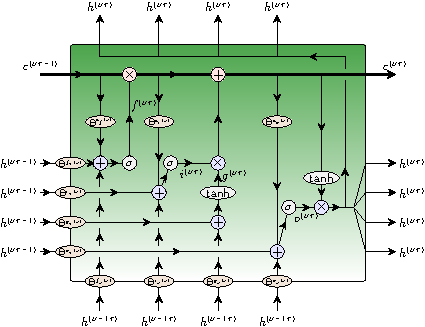
\includegraphics[scale=1.4]{LSTM_structure-peephole}};
\end{tikzpicture}
\caption{\label{fig:peepholeLSTM}LSTM hidden unit with peephole}
\end{center}
\end{figure}

Peepholes modify the gate updates in the following way

\begin{align}
i^{(\nu\tau)(t)}_f&=\sigma\left(\sum_{f'=0}^{F_{{\nu-1}}-1}\Theta^{i_{_\nu}(\nu)f}_{f'}
%
h^{(\nu-1\tau)(t)}_{f'}+\sum_{f'=0}^{F{_{\nu}}-1}\left[\Theta^{i_{_\tau}(\nu)f}_{f'}
%
h^{(\nu\tau-1)(t)}_{f'}+\Theta^{c_{_i}(\nu)f}_{f'}c^{(\nu\tau-1)(t)}_{f'}\right]\right)\;,\\
%
f^{(\nu\tau)(t)}_f&=\sigma\left(\sum_{f'=0}^{F{_{\nu-1}}-1}\Theta^{f_{_\nu}(\nu)f}_{f'}
%
h^{(\nu-1\tau)(t)}_{f'}+\sum_{f'=0}^{F_{{\nu}}-1}\left[\Theta^{f_{_\tau}(\nu)f}_{f'}
%
h^{(\nu\tau-1)(t)}_{f'}+\Theta^{c_{_f}(\nu)f}_{f'}c^{(\nu\tau-1)(t)}_{f'}\right]\right)\;,\\
%
o^{(\nu\tau)(t)}_f&=\sigma\left(\sum_{f'=0}^{F_{{\nu-1}}-1}\Theta^{o_{_\nu}(\nu)f}_{f'}
%
h^{(\nu-1\tau)(t)}_{f'}+\sum_{f'=0}^{F_{{\nu}}-1}\left[\Theta^{o_{_\tau}(\nu)f}_{f'}
%
h^{(\nu\tau-1)(t)}_{f'}+\Theta^{c_{_o}(\nu)f}_{f'}c^{(\nu\tau)(t)}_{f'}\right]\right)\;,
\end{align}
which also modifies the LSTM backpropagation algorithm in a non-trivial way. As it as been shown that different LSTM formulations lead to pretty similar results, we leave to the reader the derivation of the backpropagation update rules as an exercise.

\end{subappendices}
